\subsection{テスト技法}
\term{テスト技法}{Test Technique}は、テストケースをどの考え方で選ぶかを定める。代表的には、仕様から選ぶ仕様ベース技法、内部構造から選ぶ構造ベース技法、経験から選ぶ経験ベース技法がある。さらに、欠陥モデル、利用モデル、アプリケーションの性質、他領域から得た知識に基づく技法もある。

\par\smallskip
\begin{center}
\centering
\IfFileExists{assets/generated_figures/ch05/fig-ch05-06.png}{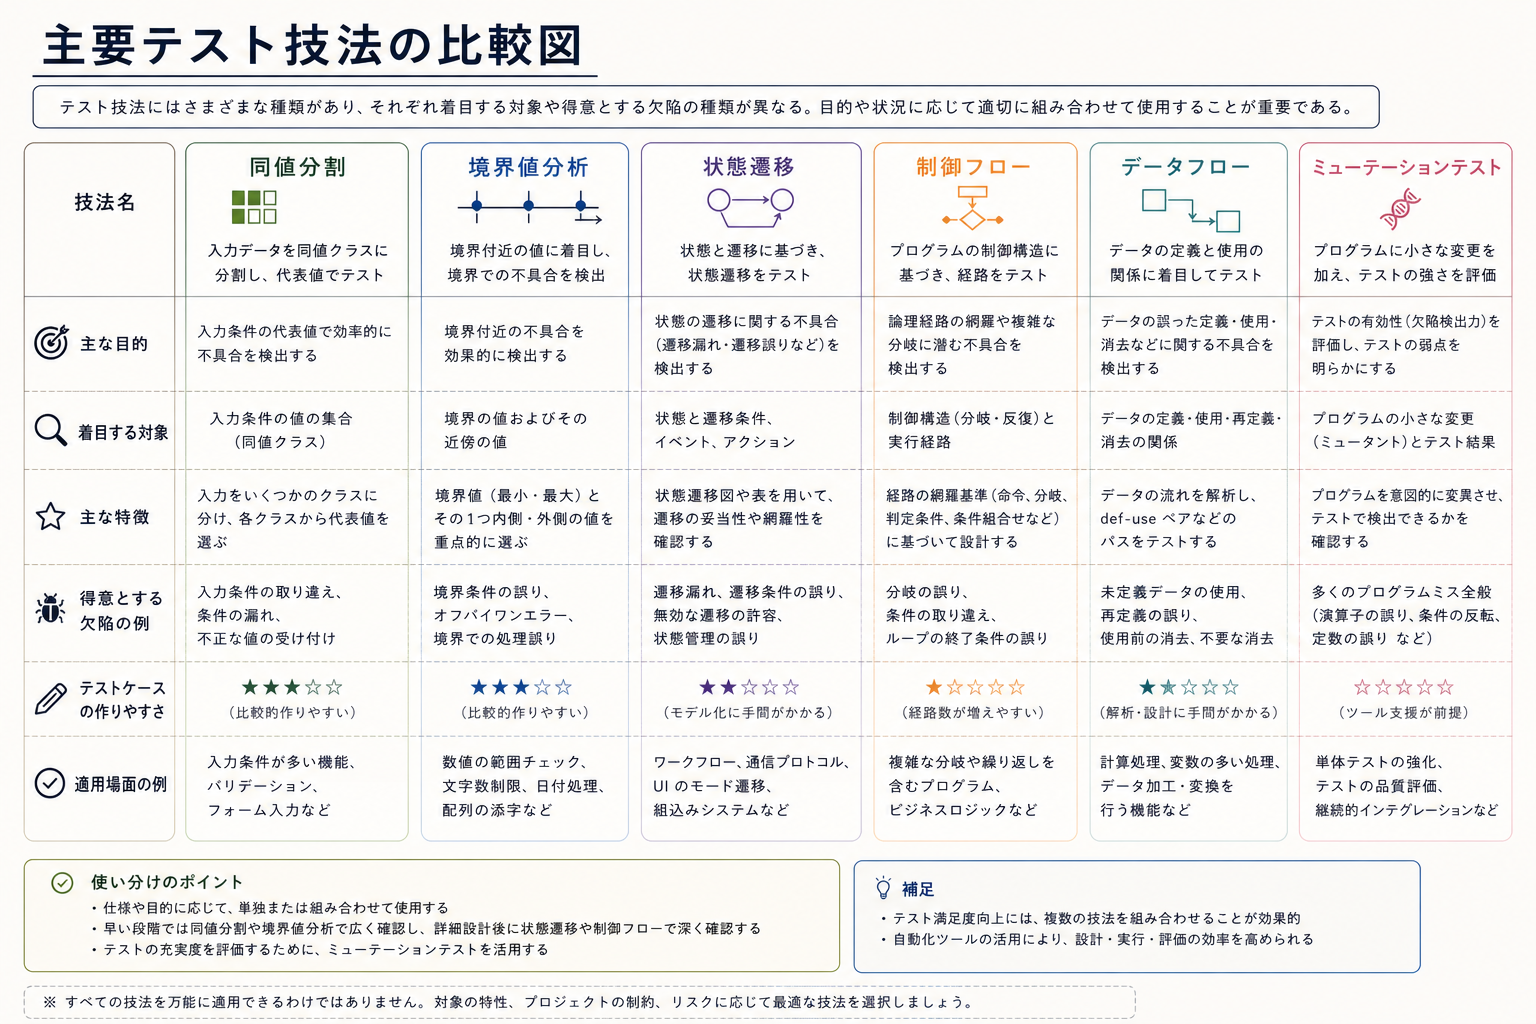
\includegraphics[width=0.96\linewidth]{assets/generated_figures/ch05/fig-ch05-06.png}}{\fbox{\parbox[c][48mm][c]{0.9\linewidth}{\centering 画像生成待ち\\主要テスト技法の比較図}}}
\par\smallskip
\refstepcounter{figure}\label{fig:ch05-06}図 \thefigure: 主要テスト技法の比較図
\end{center}
図 \thefigure は、主要テスト技法の比較図を視覚的に整理したものである。
\par\smallskip

\subsubsection{仕様ベース技法}
仕様ベース技法は、SUT の入力と出力、要求、仕様、モデルに基づいてテストケースを選ぶ。内部コードを知らなくても使えるため、ブラックボックス技法とも呼ばれる。

\paragraph{同値分割}
同値分割は、入力領域を同じように扱えると考えられる部分集合に分け、各集合から代表値を選ぶ技法である。たとえば、年齢が 0 から 120 まで有効なら、有効範囲、下限未満、上限超過などに分ける。目的は、無数の入力を少数の代表例に縮約することである。

\paragraph{境界値分析}
境界値分析は、入力範囲の境界付近に欠陥が集中しやすいという経験に基づき、下限、上限、その直前直後を選ぶ技法である。範囲外の値を使って堅牢性を見る場合もある。

\par\smallskip
\begin{center}
\centering
\IfFileExists{assets/generated_figures/ch05/fig-ch05-07.png}{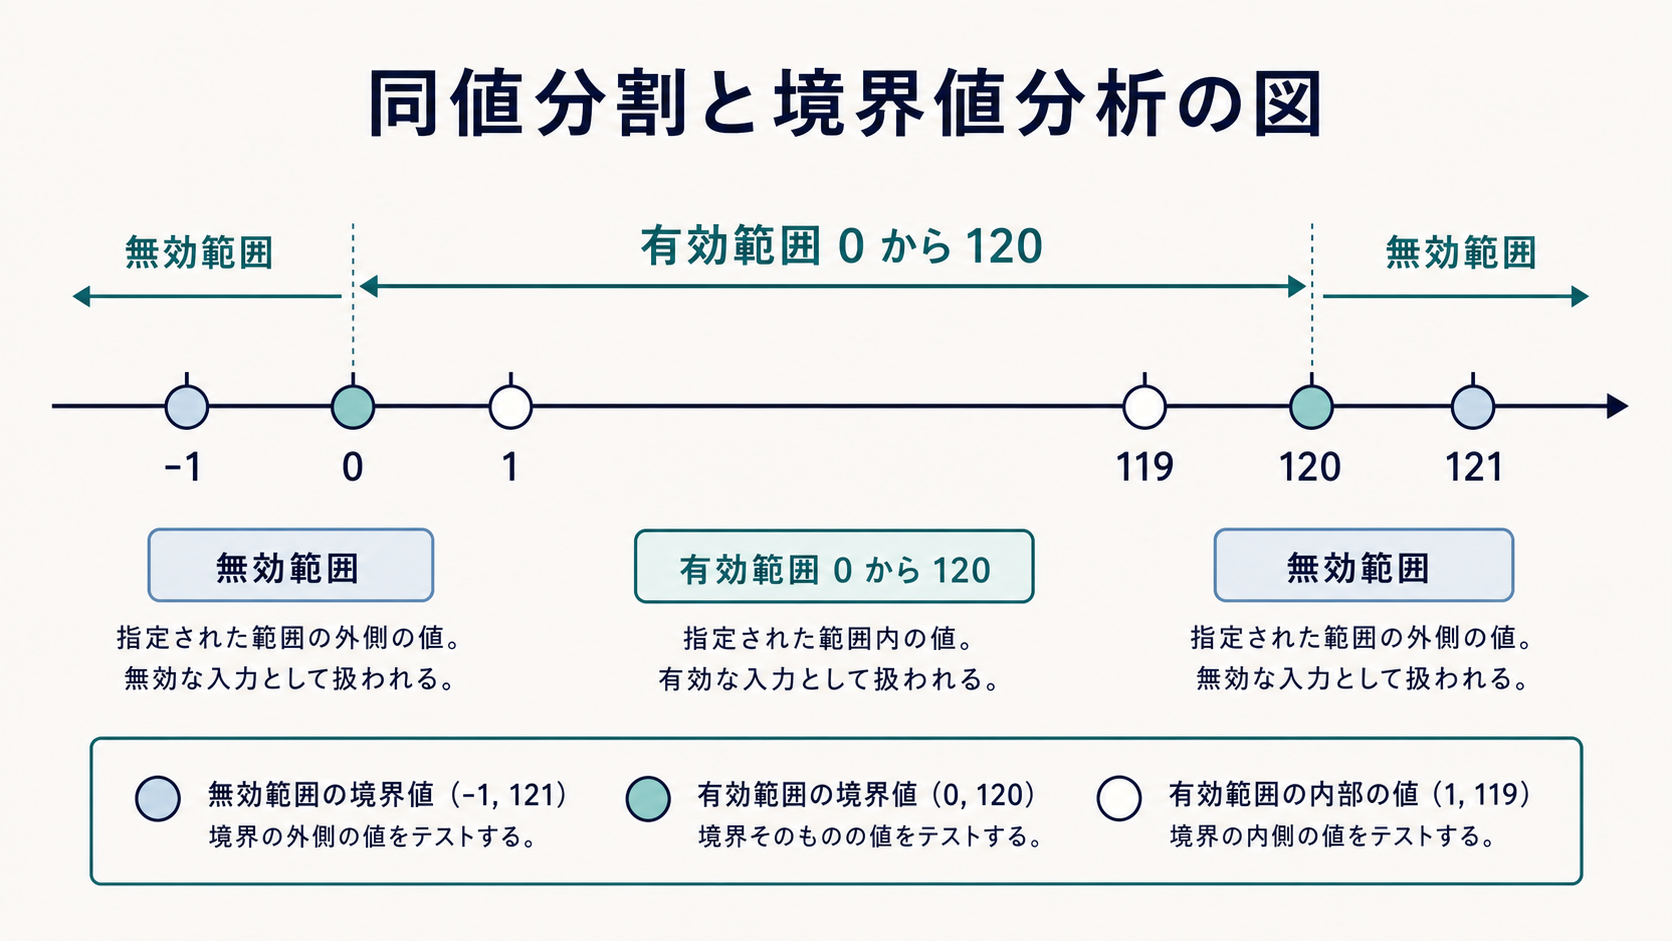
\includegraphics[width=0.96\linewidth]{assets/generated_figures/ch05/fig-ch05-07.png}}{\fbox{\parbox[c][48mm][c]{0.9\linewidth}{\centering 画像生成待ち\\同値分割と境界値分析の図}}}
\par\smallskip
\refstepcounter{figure}\label{fig:ch05-07}図 \thefigure: 同値分割と境界値分析の図
\end{center}
図 \thefigure は、同値分割と境界値分析の図を視覚的に整理したものである。
\par\smallskip

\paragraph{構文テスト}
構文テストは、形式言語で書かれた仕様や入力文法に基づいてテストケースを導く技法である。仕様が形式的であれば、機能テストケースの自動生成や期待結果の判定に使いやすい。

\paragraph{組合せテスト技法}
組合せテストは、入力値や条件の組合せを体系的に選ぶ技法である。すべての組合せを試すと数が爆発するため、ペアワイズテストのように、任意の二つのパラメータの組合せはすべて含めるという基準を使うことが多い。

\paragraph{決定表}
決定表は、条件と動作の組合せを表にして、論理関係を明示する技法である。複数条件によって結果が変わる業務規則に向いている。各条件組合せからテストケースを導けるため、抜け漏れの発見にも役立つ。

\paragraph{原因結果グラフ}
原因結果グラフは、入力条件である原因と、出力や動作である結果の関係を論理グラフとして表す技法である。仕様分析、入力条件の整理、結果条件の特定に役立つ。

\paragraph{状態遷移テスト}
状態遷移テストは、SUT を有限状態機械として表し、状態と遷移をカバーするようにテストケースを作る技法である。画面遷移、通信プロトコル、注文状態、予約状態など、状態によって振る舞いが変わる対象に向いている。

\par\smallskip
\begin{center}
\centering
\IfFileExists{assets/generated_figures/ch05/fig-ch05-08.png}{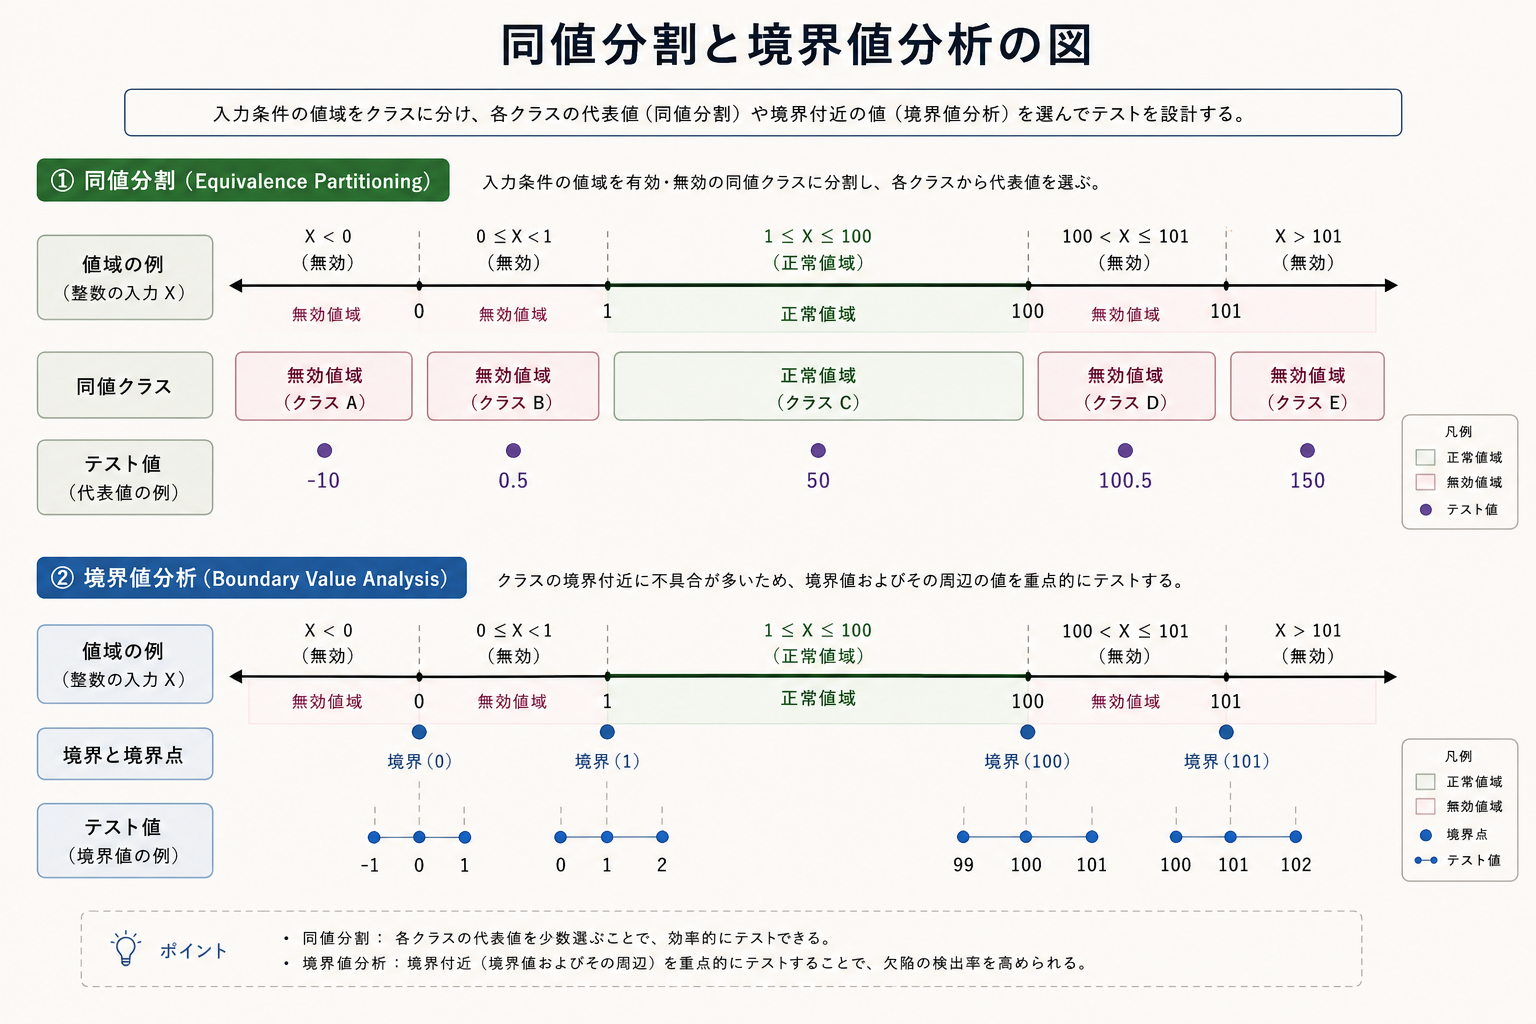
\includegraphics[width=0.96\linewidth]{assets/generated_figures/ch05/fig-ch05-08.png}}{\fbox{\parbox[c][48mm][c]{0.9\linewidth}{\centering 画像生成待ち\\状態遷移テストの図}}}
\par\smallskip
\refstepcounter{figure}\label{fig:ch05-08}図 \thefigure: 状態遷移テストの図
\end{center}
図 \thefigure は、状態遷移テストの図を視覚的に整理したものである。
\par\smallskip

\paragraph{シナリオベーステスト}
シナリオベーステストは、利用者やシステムがたどる一連の行動をモデル化し、その流れに沿ってテストケースを作る技法である。通常の流れだけでなく、代替流、例外流も扱う。業務プロセステストやワークフローモデルを使うテストもこの考え方に含まれる。

\paragraph{ランダムテスト}
ランダムテストは、入力領域からランダムにテストケースを選ぶ技法である。単純な自動化に向いているが、入力領域がわかっている必要がある。不正入力や予期しないデータを大量に与えるファズテストは、セキュリティ分野でよく用いられる。

\paragraph{証拠に基づく技法}
証拠に基づく技法は、厳密な調査手順で得た知見をテストに反映する考え方である。問いを立て、利用できる証拠を集め、批判的に分析する。体系的マッピング研究や体系的レビューは、既存研究や実務知見を整理する手段である。

\paragraph{例外強制テスト}
例外強制テストは、データ例外、操作例外、オーバーフロー、保護例外、アンダーフローなど、あらかじめ決めた例外やエラーを SUT が扱えるかを確認する。多くの場合、負のシナリオを使い、エラーメッセージや回復動作を確認する。

\subsubsection{構造ベーステスト技法}
構造ベース技法は、コードや設計の内部構造を情報源としてテストケースを選ぶ。ホワイトボックス技法とも呼ばれる。文カバレッジ、分岐カバレッジ、経路カバレッジ、循環的複雑度などが関係する。

\paragraph{制御フローテスト}
制御フローテストは、文、分岐、判定、条件、条件組合せ、経路を対象に、どの部分を実行したかを確認する。最も強い基準の一つはすべての入口から出口までの経路を通す経路テストであるが、ループがあると現実的でないため、文カバレッジ、分岐カバレッジ、条件判定カバレッジなどの基準が使われる。

\paragraph{データフローテスト}
データフローテストは、変数の定義、使用、未定義化に注目する。ある変数が定義された後、どの経路でどの使用に届くかを確認する。定義と使用の組合せを扱うため、データに関する隠れた欠陥を見つけやすい。

\paragraph{構造ベース技法の参照モデル}
構造ベース技法では、制御フローグラフがよく使われる。ノードは文や文列を表し、辺は制御の移動を表す。この図に基づいて、どの文、分岐、経路を通したかを可視化できる。

\par\smallskip
\begin{center}
\centering
\IfFileExists{assets/generated_figures/ch05/fig-ch05-09.png}{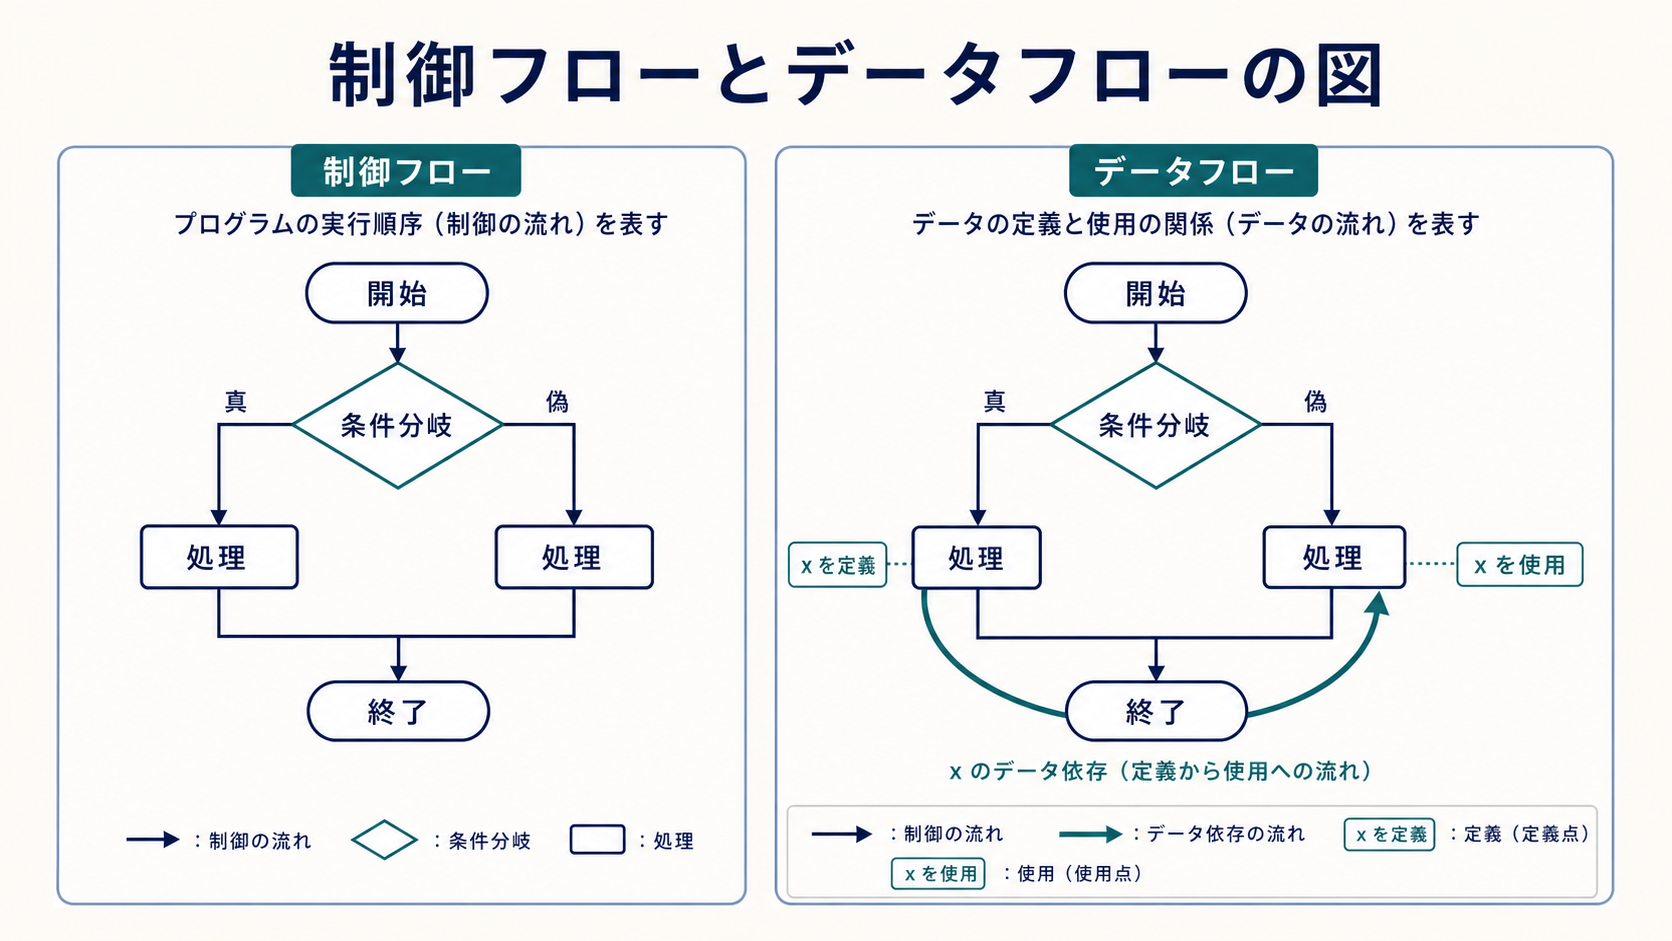
\includegraphics[width=0.96\linewidth]{assets/generated_figures/ch05/fig-ch05-09.png}}{\fbox{\parbox[c][48mm][c]{0.9\linewidth}{\centering 画像生成待ち\\制御フローとデータフローの図}}}
\par\smallskip
\refstepcounter{figure}\label{fig:ch05-09}図 \thefigure: 制御フローとデータフローの図
\end{center}
図 \thefigure は、制御フローとデータフローの図を視覚的に整理したものである。
\par\smallskip

\subsubsection{経験ベース技法}
経験ベース技法は、仕様やコードだけではなく、テスト担当者の知識、直感、過去の障害、ドメイン理解を活用する。

\paragraph{エラー推測}
エラー推測は、過去の欠陥履歴や経験に基づき、「ここに欠陥がありそうだ」と考えてテストケースを設計する技法である。形式的な技法では見つけにくい問題を見つけることがある。

\paragraph{探索的テスト}
探索的テストは、学習、テスト設計、テスト実行を同時に進める活動である。事前にすべてのテストケースを決めるのではなく、観測した振る舞い、リスク、失敗の兆候に基づいて次のテストを考える。要求が詳細でないアジャイル開発などでよく使われる。

\paragraph{その他の経験ベース技法}
アドホックテストは、技能、直感、経験に基づいてテストする。モンキーテストはランダムな操作で停止や異常を狙う。ペアテストは二人でテストを行い、一人が操作し、一人が観察する。ゲーミフィケーションは、テスト作業をゲーム要素に変換して参加を促す。クイックテストは小さなテストスイートで重大問題を早く見つける。スモークテストは、ビルド後に基本機能が動くかを確認し、本格的なテストに進める状態かを判断する。

\subsubsection{欠陥ベース技法とミューテーション技法}
欠陥ベーステストは、あり得る欠陥の種類を想定し、それを露出させるテストケースを作る。欠陥分類や直交欠陥分類を使うと、欠陥の意味情報を整理し、根本原因分析を短縮できる。

ミューテーションテストは、SUT をわずかに変更した変異体を多数作り、テストスイートがそれらの違いを検出できるかを評価する技法である。テストが変異体を見破れば、その変異体は殺されたという。変異体を多く殺せるテストスイートほど、欠陥検出能力が高いと考える。近年は、機械学習システムのテストで、入力を変化させて出力関係を見るメタモルフィックテストにも関連する。

\par\smallskip
\begin{center}
\centering
\IfFileExists{assets/generated_figures/ch05/fig-ch05-10.png}{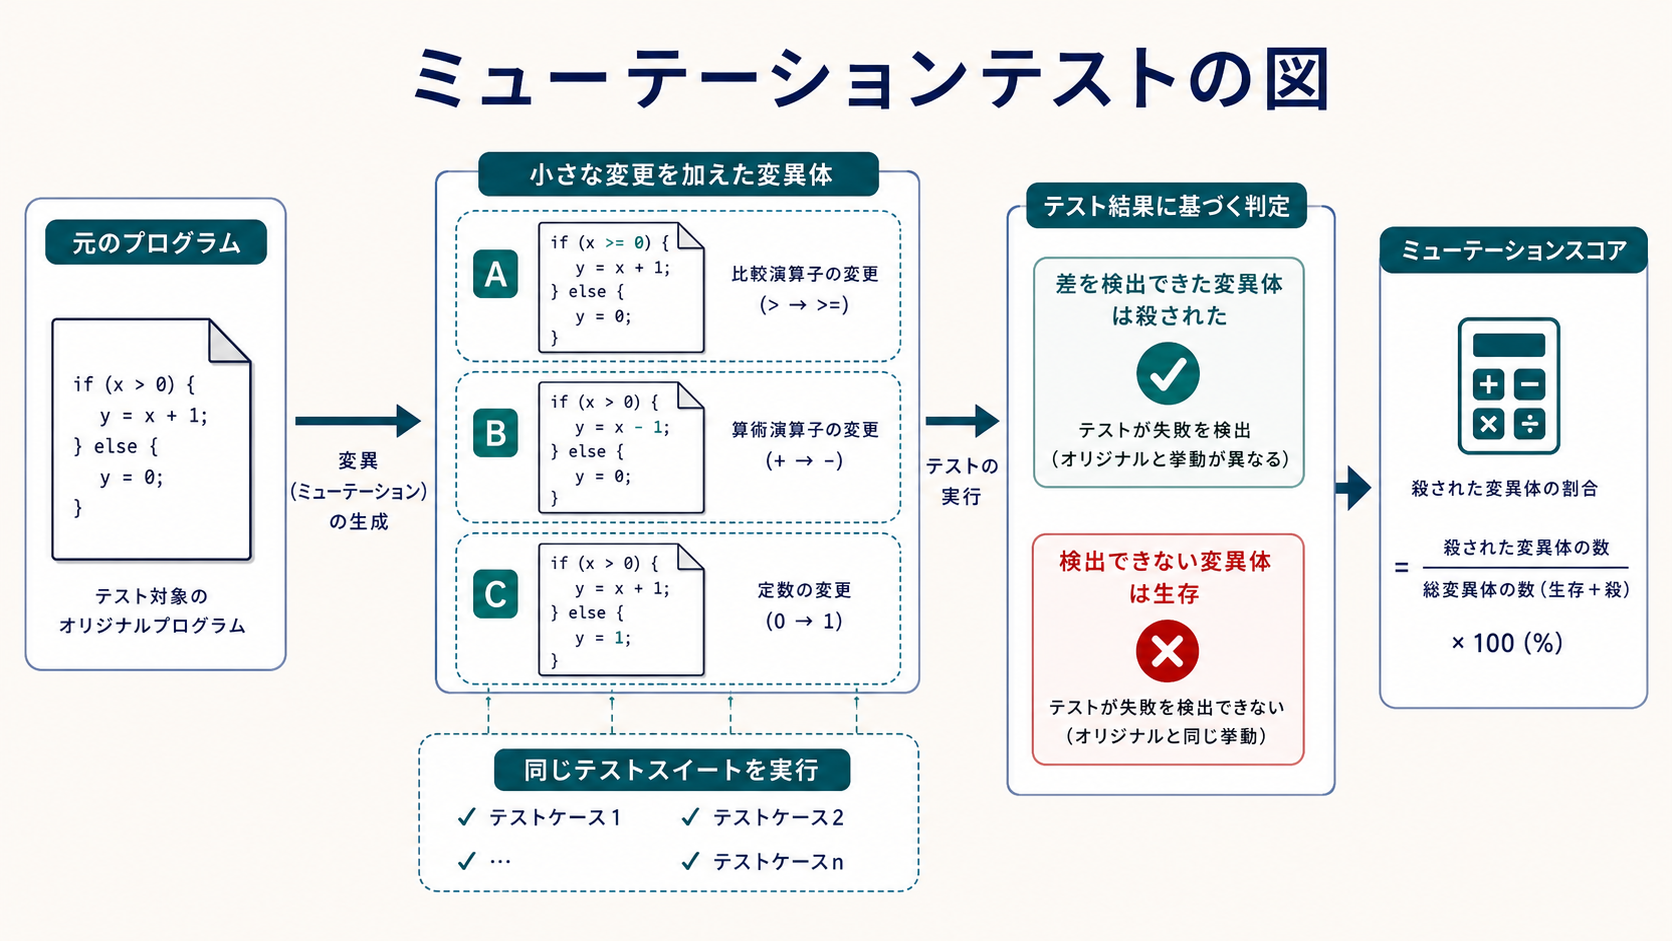
\includegraphics[width=0.96\linewidth]{assets/generated_figures/ch05/fig-ch05-10.png}}{\fbox{\parbox[c][48mm][c]{0.9\linewidth}{\centering 画像生成待ち\\ミューテーションテストの図}}}
\par\smallskip
\refstepcounter{figure}\label{fig:ch05-10}図 \thefigure: ミューテーションテストの図
\end{center}
図 \thefigure は、ミューテーションテストの図を視覚的に整理したものである。
\par\smallskip

\subsubsection{利用ベース技法}
利用ベース技法は、実際の運用や利用のされ方をモデル化し、その頻度や順序に沿ってテストケースを選ぶ。運用環境に近い条件で実行するため、受入テストや信頼性評価に向いている。

\paragraph{運用プロファイル}
運用プロファイルは、入力や利用シナリオが実運用でどの頻度で起こるかを表す。運用プロファイルに基づくテストでは、観測した結果から将来の信頼性を推定する。難しさは、現実的なプロファイルを作ることにある。

\paragraph{利用者観察ヒューリスティック}
利用者観察ヒューリスティックは、利用者がシステムやインタフェースをどれだけうまく使えるかを、統制された条件で観察する。認知的ウォークスルー、発話思考法、現場観察、質問票、面接などが使われる。

\subsubsection{アプリケーションの性質に基づく技法}
一般的な技法は多くのソフトウェアに使えるが、対象の性質によって追加の技法が必要になる。オブジェクト指向ソフトウェア、コンポーネントベースソフトウェア、ウェブアプリケーション、並行プログラム、通信プロトコル、リアルタイムシステム、安全重要システム、サービス指向ソフトウェア、オープンソース、組込み、クラウド、ブロックチェーン、ビッグデータ、AI・機械学習、モバイル、セキュリティ・プライバシー重視ソフトウェアなどでは、対象特有のリスクを考慮する。

\subsubsection{技法の選択と組合せ}
実務では、一つの技法だけで十分な品質根拠を得ることは少ない。仕様ベースと構造ベースを組み合わせれば、外部振る舞いと内部網羅を両方確認できる。リスクが高い部分には手厚い技法を使い、低リスク部分には軽量な技法を使うなど、目的、費用、リスク、組織制約に応じて選ぶ。

\paragraph{機能的技法と構造的技法の組合せ}
シナリオベーステストは機能的観点を強く持つ。構造ベーステストは内部構造の観点を強く持つ。両者は対立ではなく補完関係である。仕様に書かれた動作を確認しつつ、実装上の分岐やデータ流れも確認することで、見落としを減らせる。

\paragraph{決定的テストとランダムテスト}
決定的テストは、基準に従って選ばれたテストケースを実行する。ランダムテストは、確率分布に従って入力を選ぶ。信頼性テストではランダム性が役立つことがあるが、境界や特定リスクを狙う場合には決定的な選択が有効である。

\subsubsection{派生知識に基づく技法}
派生知識に基づく技法は、他の研究領域や文脈から得られた知識をテストに取り入れる。デジタルツイン、シミュレーション、機械学習、ゲーミフィケーション、模擬ニューラルネットワークなどが例である。テスト活動を支援し、効果を高めることを目的とする。
